\apendice{Documentación de usuario}

\section{Introducción}
En este apartado se detallarán las principales funcionalidades que ofrece la aplicación de escritorio a si como todo lo necesario para que los usuarios puedan instalar y ejecutar la aplicación fácilmente. 

\section{Requisitos de usuarios}
Para poder correr la aplicación será necesario tener instalado \textit{Python}, al menos la versión 3.8.8 e instalar los requerimientos especificados en el fichero \texttt{app/requirements.txt}. Esta aplicación está pensada para ser ejecutada sobre el sistema operativo \textit{Windows}.

\section{Instalación}
Los pasos básicos para instalar el proyecto y con ende la aplicación son los siguientes:
\begin{enumerate}
    \item Clonar repositorio e ir al directorio \texttt{app/}.
    \item Comprobar que se encuentran almacenados algunos vídeos en las diferentes carpetas que contiene el directorio \texttt{app/}.
    \item Ejecutar el comando:
    \newpage
    \begin{lstlisting}[language=Bash]
 Sintaxis
        install.cmd 
    \end{lstlisting}
    o en su defecto
    \begin{lstlisting}[language=Bash]
 Sintaxis
        pip install -r requirements.txt
    \end{lstlisting}
\end{enumerate}

Finalmente para ejecutar la aplicación:
Para ejecutar la aplicación:
\begin{lstlisting}[language=Bash]
 Sintaxis
    python main.py
\end{lstlisting}


\section{Manual del usuario}

\subsection{Cambiar el modo de la aplicación}
Para cambiar el modo de la aplicación observar figuras \ref{fig:app1} \ref{fig:app2}. Al cambiar de modo se ejecutarán las siguientes acciones:
\begin{enumerate}
    \item \textbf{Cambio de colores}: si el usuario se encuentra en \textit{modo ejemplo ON} aparecerá una ventana con tonos verdes azulados y azules, mientras que si el usuario se encuentra en \textit{modo ejemplo OFF} los tonos serán de color lila. Al cambiar el color de toda la aplicación dependiendo del modo de ejecución en el que se encuentre el usuario se logra evitar confusiones sobre en que modo se encuentra. 
    \item \textbf{Cambio del texto del botón}: es imprescindible que el usuario sepa en todo momento en que modo de ejecución se encuentra por lo que el cambio de colores no es suficiente, mediante el botón \textit{ON/OFF} se informará del modo en el que se encuentra la aplicación. 
    \item \textbf{Bloqueo o desbloqueo de casillas}: las casillas por las que se inserta el \textit{frame} de inicio y final aparecerán bloqueadas si el usuario se encuentra en \textit{modo ejemplo ON} ya que no necesitará hacer uso de ellas.
    \item \textbf{Actualización de vídeos}: si la aplicación cambia de modo, se actualizarán los vídeos mostrados en las listas de selección. Cada modo puede contener diferentes vídeos.
    \item \textbf{Descarte de vídeos}: si la aplicación está reproduciendo un vídeo y se ejecuta un cambio de modo, automáticamente descartará el vídeo.
\end{enumerate}

\begin{figure}[H]
    \centering
    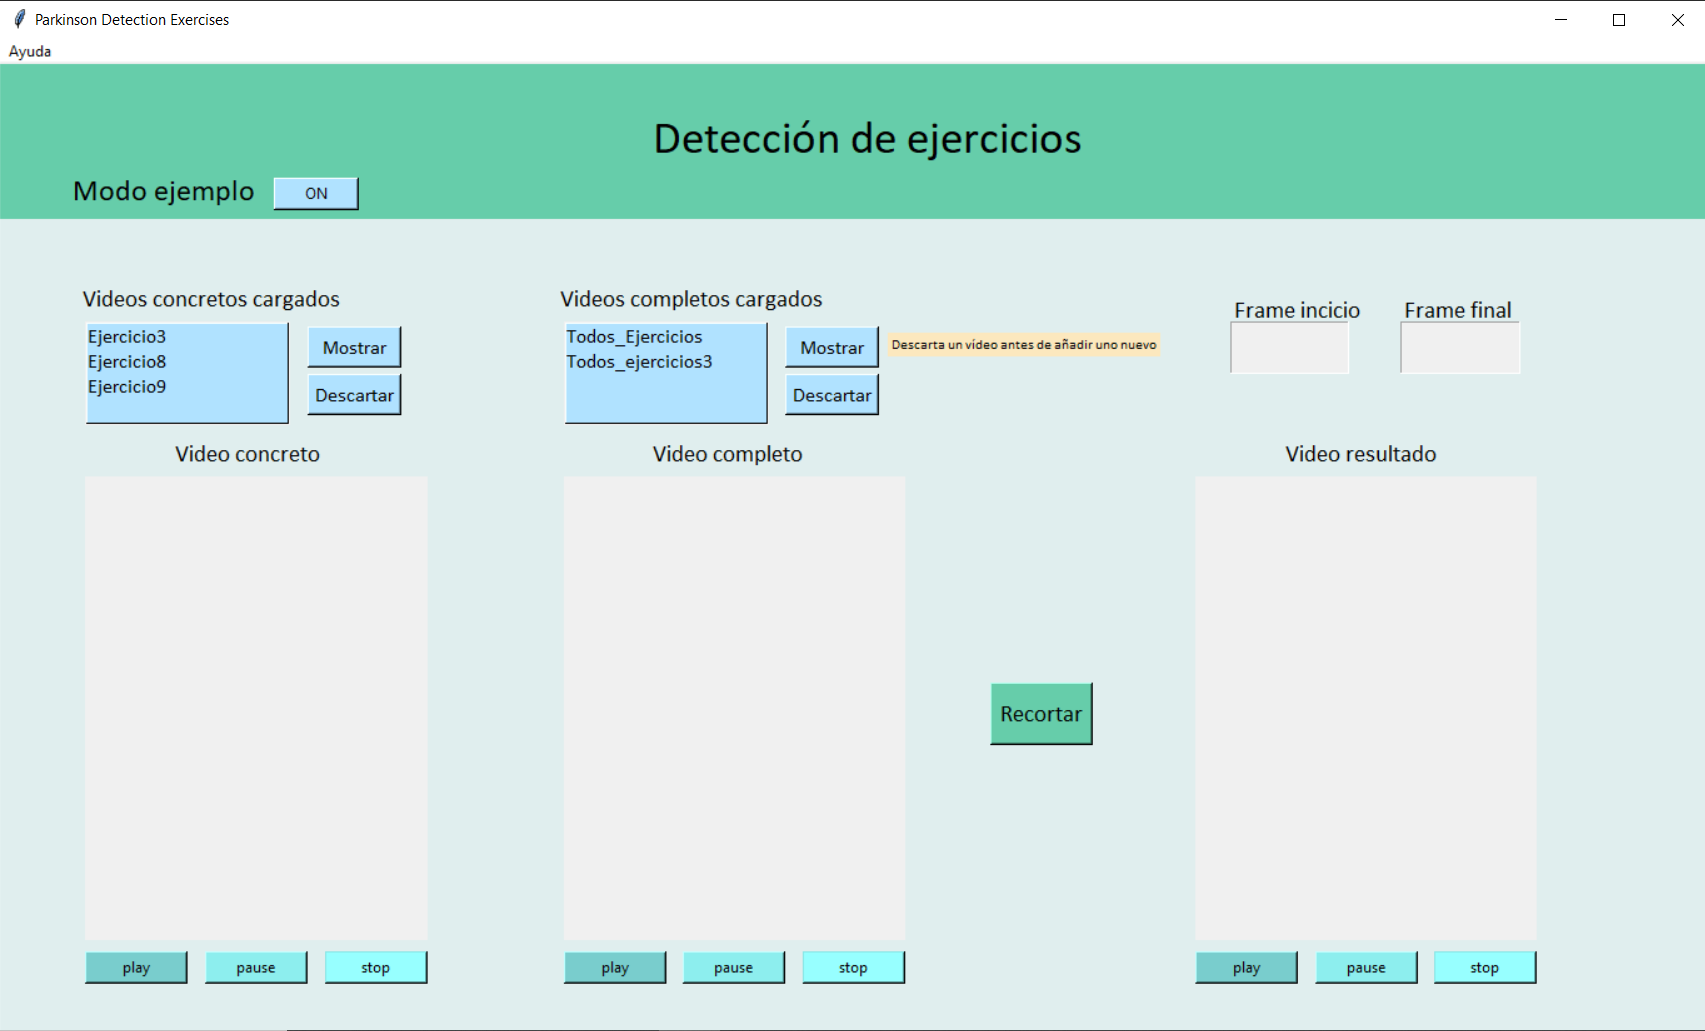
\includegraphics[width=0.8\textwidth]{plantillaLatex-master/img/app1.PNG}
    \caption{Aplicación en modo ejemplo ON.}
    \label{fig:app1}
\end{figure}

\begin{figure}[H]
    \centering
    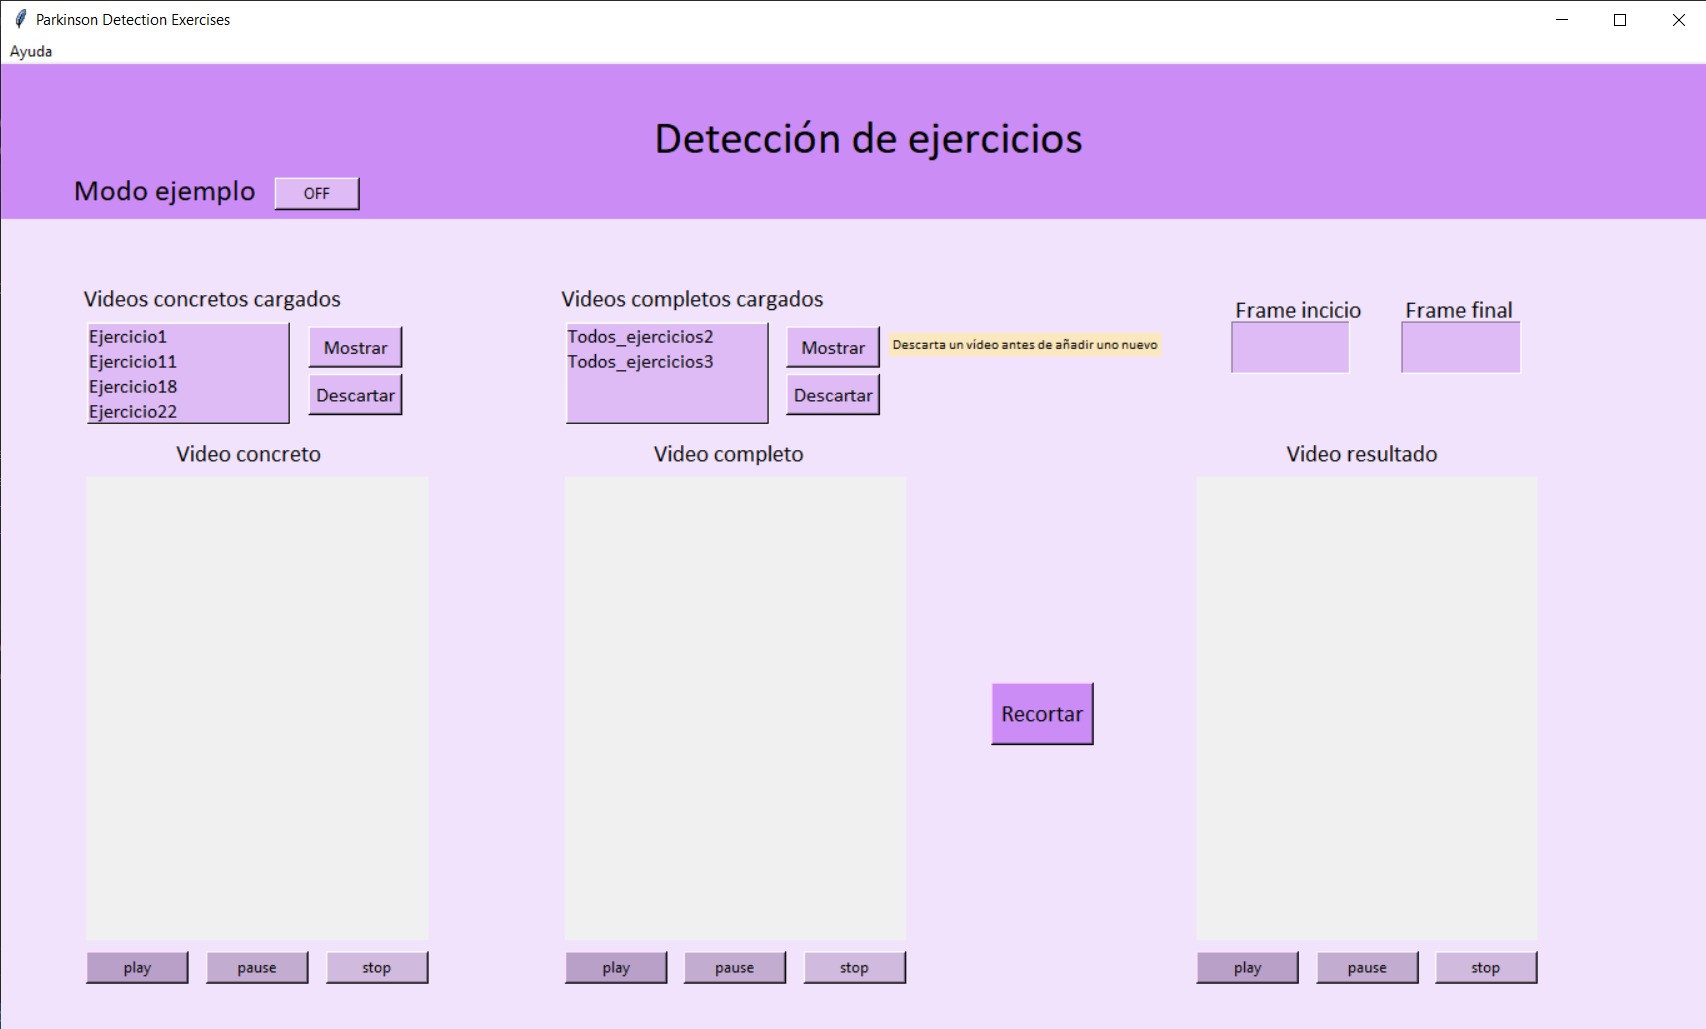
\includegraphics[width=0.8\textwidth]{plantillaLatex-master/img/app2.PNG}
    \caption{Aplicación en modo ejemplo OFF.}
    \label{fig:app2}
\end{figure}

\subsection{Mostrar y borrar un vídeo}
Una vez se arranca la aplicación de escritorio, los vídeos son cargados automáticamente por la aplicación y mostrados en la barra de selección. 

\subsubsection{Mostrar un vídeo}
Para mostrar un vídeo ver figura \ref{fig:app3}. Al mostrar un vídeo se ejecutarán las siguientes acciones:
\begin{enumerate}
    \item \textbf{Seleccionar un vídeo}: lo primero que se deberá hacer es escoger un vídeo de los mostrados en la lista de selección.
    \item \textit{Pinchar en el botón \textbf{Mostrar}}: tras seleccionar un vídeo y seguidamente pinchar en este botón, la aplicación cargará el vídeo seleccionado en su ventana correspondiente y empezará con su reproducción. 
    \item \textbf{Descartar vídeos previos}: si se desea cargar un vídeo cuando ya hay otro en ejecución, es muy importante descartar el vídeo previo. En caso de no realizarse correctamente esta acción, el vídeo seleccionado no se cargará.
\end{enumerate}

\begin{figure}[H]
    \centering
    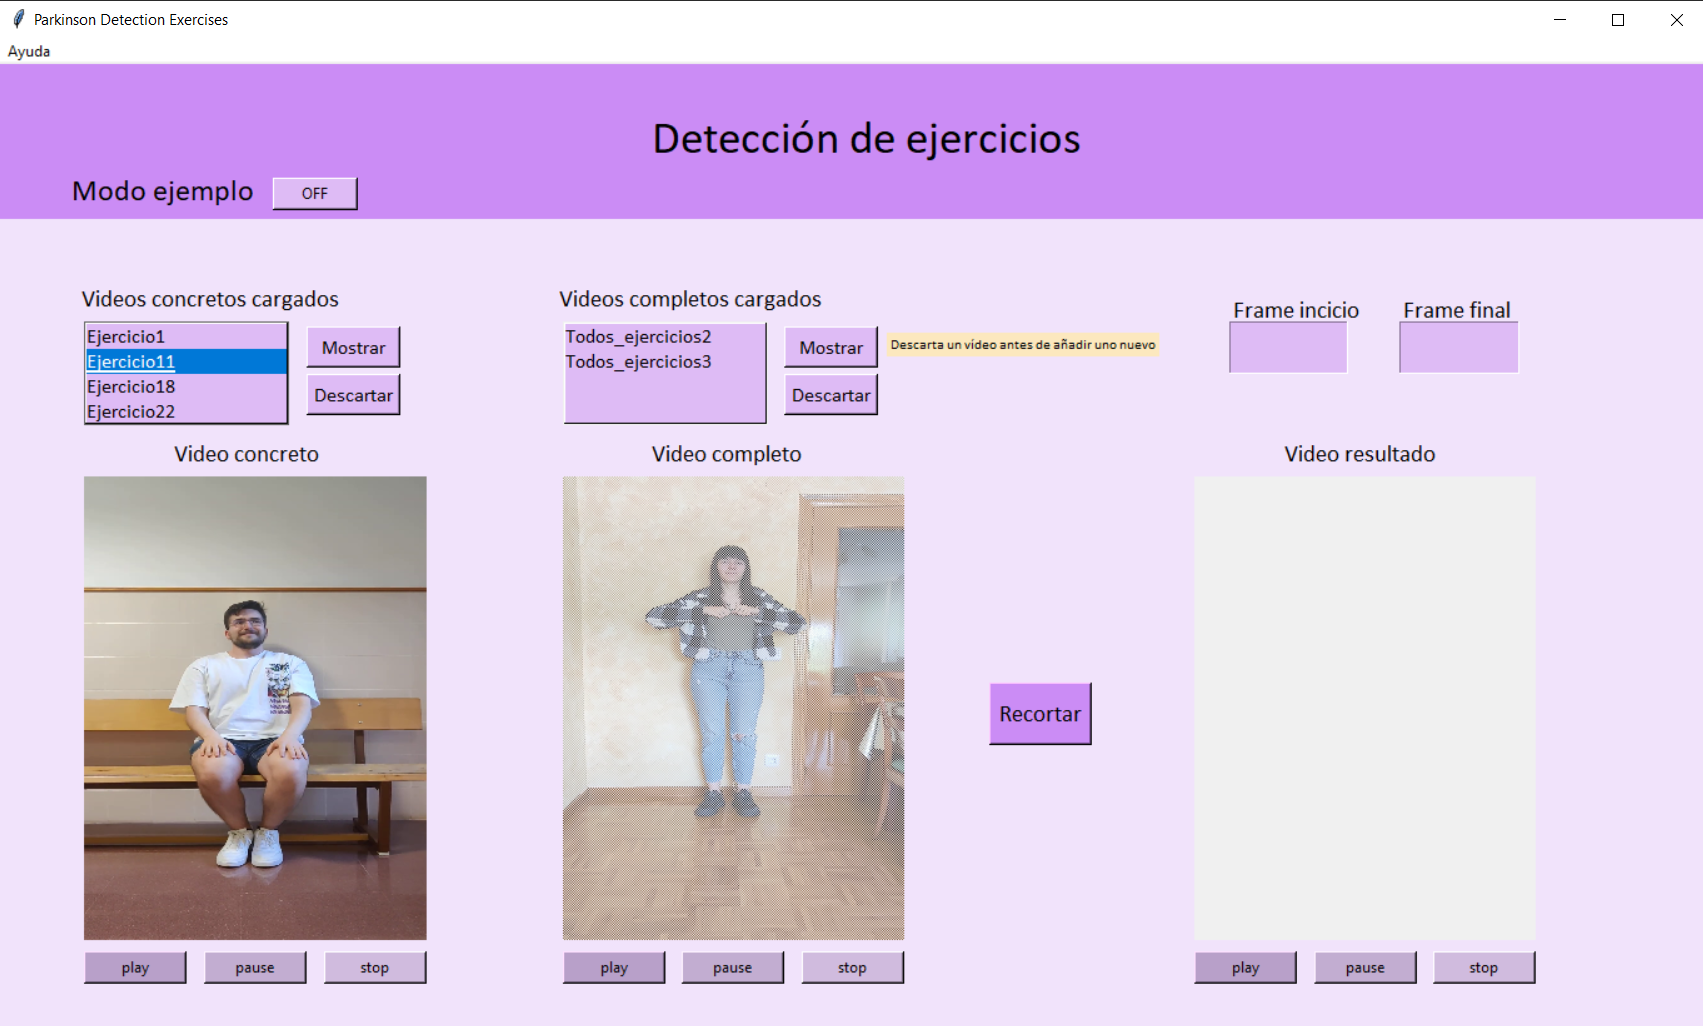
\includegraphics[width=\textwidth]{plantillaLatex-master/img/app3.PNG}
    \caption{Carga y descarte de vídeos.}
    \label{fig:app3}
\end{figure}

\subsubsection{Descartar un vídeo}
Para descartar un vídeo ver figura \ref{fig:app3}. Al descartar un vídeo se ejecutarán las siguientes acciones:
\begin{enumerate}
    \item \textbf{Seleccionar el vídeo}: para que el vídeo se descarte correctamente se deberá seleccionar el vídeo que está en ejecución y que se desea eliminar. 
    \item \textbf{Pinchar en el botón \textit{Descartar}}: una vez seleccionado el vídeo se pulsará este botón. Esta acción simplemente deja de reproducirlo en su ventana correspondiente, pero no elimina el vídeo de la lista de selección,
    por esta razón se pueden cargar y descartar tantas veces como se desee.
    \item \textbf{EL vídeo se bloqueará}: como se ha comentado anteriormente los vídeos no son eliminados por completo si no que únicamente se bloquean y dejan de reproducirse. Una vez el vídeo está bloqueado se podrán añadir nuevos vídeos.
\end{enumerate}

\subsection{Interaccionar con el vídeo}
Una vez esté cargado un vídeo, se podrá pausar y reanudar tantas veces como el usuario desee. 

\subsubsection{Reproducir un vídeo}
Para reproducir un vídeo se tendrán en cuenta estas sencillas acciones:
\begin{enumerate}
    \item \textbf{Pinchar en el botón \textit{play}}: los vídeos pausados o detenidos únicamente empezarán  a reproducirse pulsando este botón. 
    \item \textbf{EL vídeo empezará a reproducirse}: si el vídeo se encuentra pausado o detenido, ya sea porque el usuario ha presionado el botón \textit{stop} o porque la duración del vídeo ha llegado a su fin, una vez se pincha sobre el botón \textit{play}, empezará su reproducción.
\end{enumerate}

\newpage
\subsubsection{Pausar un vídeo}
Para pausar un vídeo se tendrán en cuenta estas sencillas acciones:
\begin{enumerate}
    \item \textbf{Pinchar en el botón \textit{pause}}: este botón únicamente permitirá la pausa del vídeo en reproducción. No ejecutará el vídeo de nuevo al hacer doble \textit{click}.
    \item \textbf{EL vídeo se pausará}: el vídeo permanecerá pausado hasta que se ejecute una acción de reproducción. 
\end{enumerate}

\subsubsection{Detener un vídeo}
Para detener un vídeo se tendrán en cuenta estas sencillas acciones:
\begin{enumerate}
    \item \textbf{Pinchar en el botón \textit{stop}}: este botón únicamente permitirá la detención inmediata del vídeo en reproducción. No ejecutará el vídeo de nuevo al hacer doble \textit{click}. 
    \item \textbf{EL vídeo se parará}: el vídeo permanecerá detenido hasta que se ejecute una acción de reproducción. En este caso, el vídeo comenzará desde el instante inicial.
\end{enumerate}


\subsection{Recortar un vídeo}
Los vídeos se podrán recortar en ambos modos de ejecución. En las imágenes \ref{fig:app5} y \ref{fig:app4} se puede observar como el ejercicio realizado por el vídeo que simula al terapeuta es localizado en el vídeo que simula al paciente y posteriormente muestra dicho resultado. 

\subsubsection{Recortar un vídeo en modo ejemplo ON}
Para recortar un vídeo en \textit{modo ejemplo ON} ver figura \ref{fig:app5} y tener en cuenta las siguientes acciones:
\begin{enumerate}
    \item \textbf{Seleccionar un vídeo concreto}: se deberá escoger el vídeo que se desea encontrar dentro de la secuencia de ejercicios.
    \item \textbf{Seleccionar un vídeo completo}: también se deberá escoger el vídeo del que se desea obtener el recorte.
    \item \textbf{Pinchar en el botón \textit{Recortar}}: para ver el resultado final del recorte se deberá pulsar en este botón. En cuanto el vídeo recortado sea cargado empezará a reproducirse.
\end{enumerate}
\begin{figure}[H]
    \centering
    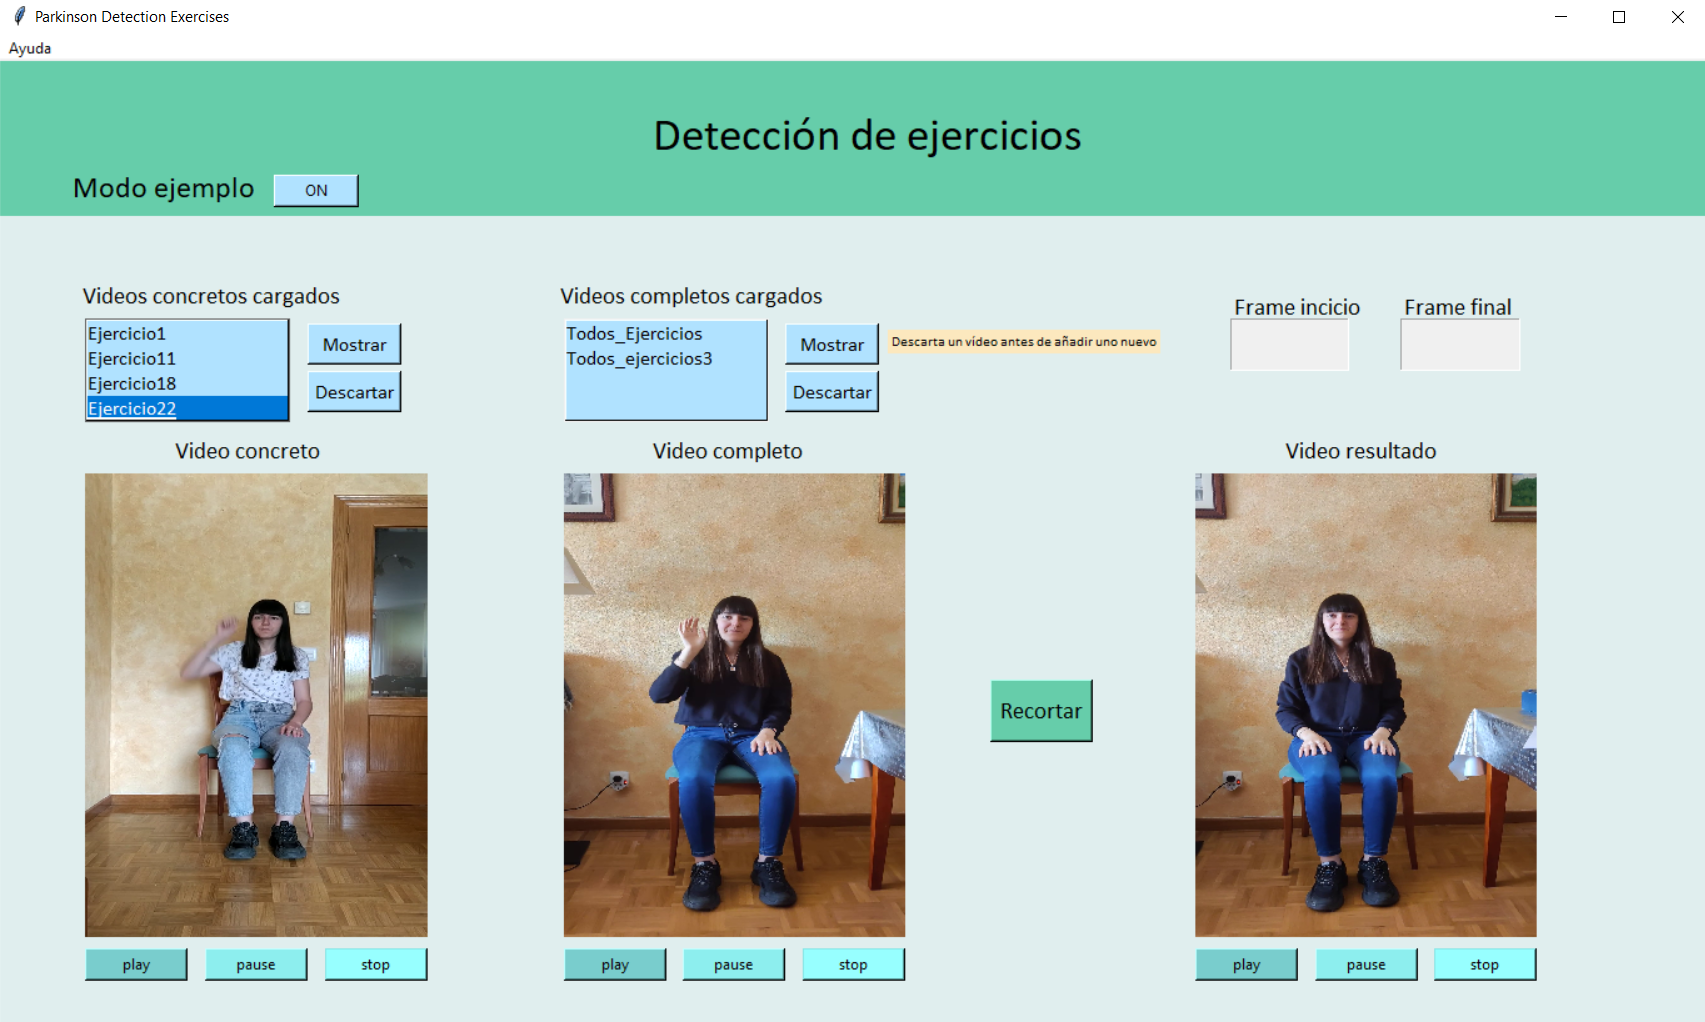
\includegraphics[width=\textwidth]{plantillaLatex-master/img/app5.PNG}
    \caption{Recorte de vídeos en modo ejemplo ON.}
    \label{fig:app5}
\end{figure}

\subsubsection{Recortar un vídeo en modo ejemplo OFF}
Para recortar un vídeo en \textit{modo ejemplo OFF} ver figura \ref{fig:app4} y tener en cuenta las siguientes acciones:
\begin{enumerate}
    \item \textbf{Seleccionar un vídeo concreto}.
    \item \textbf{Seleccionar un vídeo completo}.
    \item \textbf{Indicar el \textit{frame} de inicio}: para el generar el recorte será necesario indicar el punto de inicio en la casilla correspondiente.
    \item \textbf{Indicar el \textit{frame} de final}: también será necesario especificar el punto en el que se desea que finalice el resultado. 
    \item \textbf{Pinchar en el botón \textit{Recortar}}: una vez se tienen ambos valores cargados, tras seleccionar este botón aparecerá el vídeo resultado reproduciéndose automáticamente.
\end{enumerate}
\begin{figure}
    \centering
    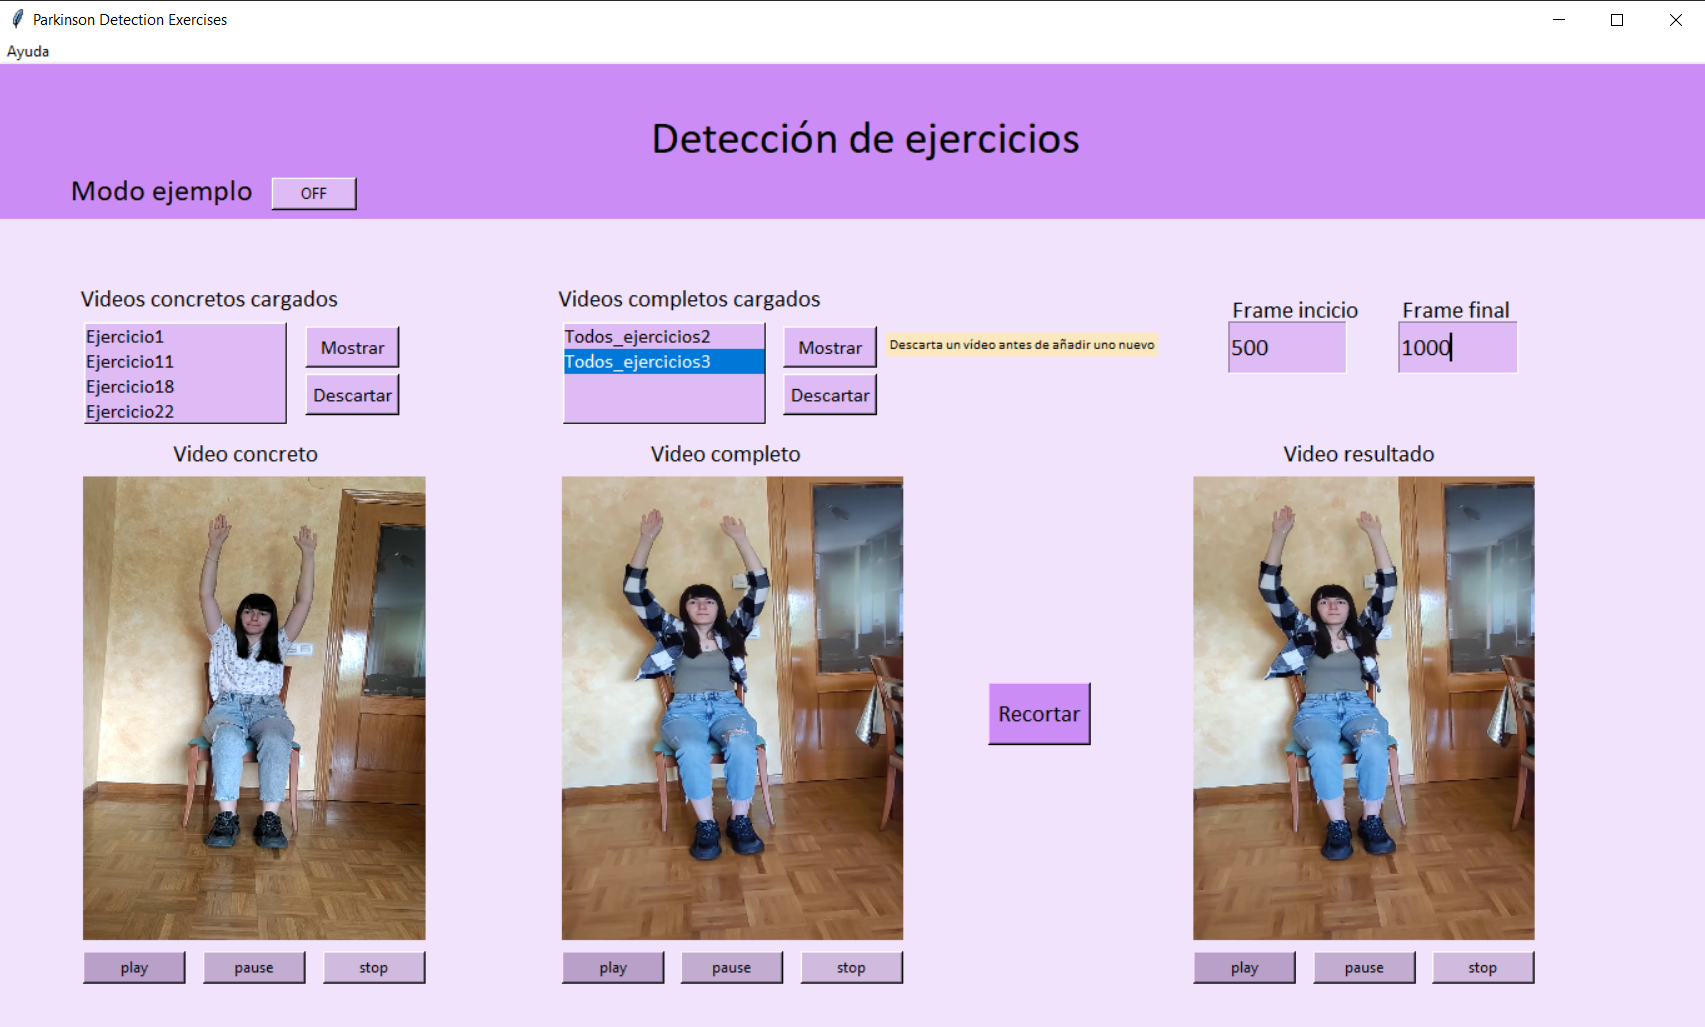
\includegraphics[width=0.9\textwidth]{plantillaLatex-master/img/app4.PNG}
    \caption{Recorte de vídeos en modo ejemplo OFF.}
    \label{fig:app4}
\end{figure}

\subsection{Excepciones e información de la aplicación}
Finalmente comentar los siguientes aspectos relevantes e la aplicación:
\begin{enumerate}
    \item Si el usuario se encuentra en el \textit{modo ejemplo ON} y selecciona el botón recortar sin haber especificado los \textit{frames} de inicio y de final, mostrará el siguiente aviso:
    \begin{figure}[H]
        \centering
        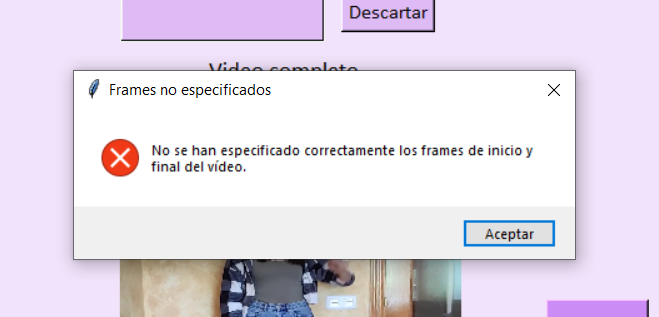
\includegraphics[width=0.35\textwidth]{plantillaLatex-master/img/NoFrames.PNG}
        \caption{Aviso de falta de frames.}
    \label{fig:app4}
\end{figure}
    \item Si se selecciona el desplegable \textbf{\textit{Ayuda}} se mostrarán las opciones \textit{Proyecto} y \textit{Modo ejemplo} que mostrarán la siguiente información:
\begin{figure}[H]
 \centering
  \subfloat {
   \label{f:gatos}
    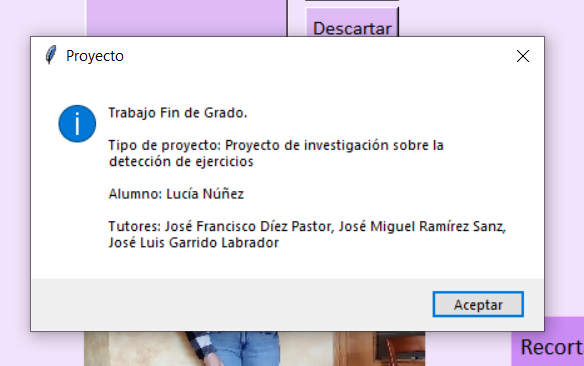
\includegraphics[width=0.295\textwidth]{plantillaLatex-master/img/ProyectInf.PNG}}
  \subfloat {
   \label{f:perros}
    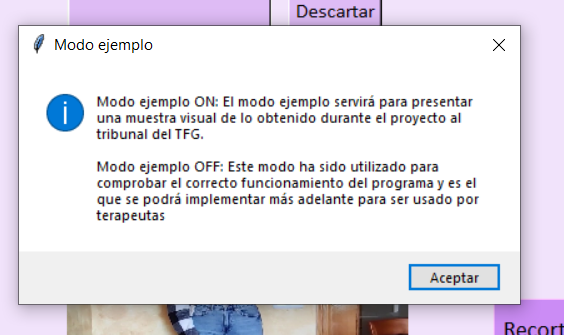
\includegraphics[width=0.32\textwidth]{plantillaLatex-master/img/ExampleMode.PNG}}
 \caption{Detección de animales usando diferentes algoritmos.}
 \label{f:animales1}
\end{figure}

    
\end{enumerate}
